\documentclass[10pt,a4paper]{article}

% --- Paquetes principales ---
\usepackage[utf8]{inputenc}
\usepackage[spanish,es-nodecimaldot]{babel}
\usepackage{amsmath,amssymb,amsfonts,amsthm}
\usepackage{geometry}
\geometry{top=1.8cm, bottom=1.8cm, left=1.8cm, right=1.8cm}
\usepackage{booktabs}
\usepackage{tabularx}
\usepackage{array}
\usepackage{xcolor}
\usepackage{hyperref}
\usepackage{bm}
\usepackage{microtype}
\usepackage{fancyhdr}
\usepackage{float}
\usepackage{graphicx}
\graphicspath{{report/}{./}{../}}
\usepackage[justification=centering, font=small, labelfont=bf]{caption}

% Permitir que las ecuaciones fluyan naturalmente entre páginas
\allowdisplaybreaks

% --- Colores y estilos ---
\definecolor{primary}{RGB}{20, 50, 95}
\definecolor{secondary}{RGB}{35, 110, 160}
\definecolor{accent}{RGB}{210, 75, 55}

\hypersetup{
    colorlinks=true,
    linkcolor=primary,
    citecolor=secondary,
    urlcolor=secondary
}

\setlength{\headheight}{14pt}
\pagestyle{fancy}
\fancyhf{}
\rhead{\textcolor{gray}{\small Tarea 1: Fundamentos de redes neuronales profundas}}
\lhead{\textcolor{gray}{\small Edwyn Guzmán -- C.I. 30.326.271}}
\cfoot{\thepage}
\renewcommand{\headrulewidth}{0.4pt}

\title{\vspace{-1.2cm}
\textbf{\LARGE Tarea 1: Fundamentos de redes neuronales profundas}\\[0.3cm]
\large Escuela de Computación, Facultad de Ciencias -- Universidad Central de Venezuela
}
\author{\textbf{Estudiante:} Edwyn Guzmán \quad (\text{C.I.} 30.326.271) \qquad \textbf{Profesor:} Fernando Crema García}
\date{Semestre I-2026}

\begin{document}

\maketitle
\thispagestyle{fancy}
\vspace{-1.0cm}
\noindent\rule{\textwidth}{0.8pt}
\vspace{0.1cm}

\section*{II-A. Backpropagation}

\subsection*{Arquitectura y parámetros iniciales de la red}

\begin{figure}[H]
    \centering
    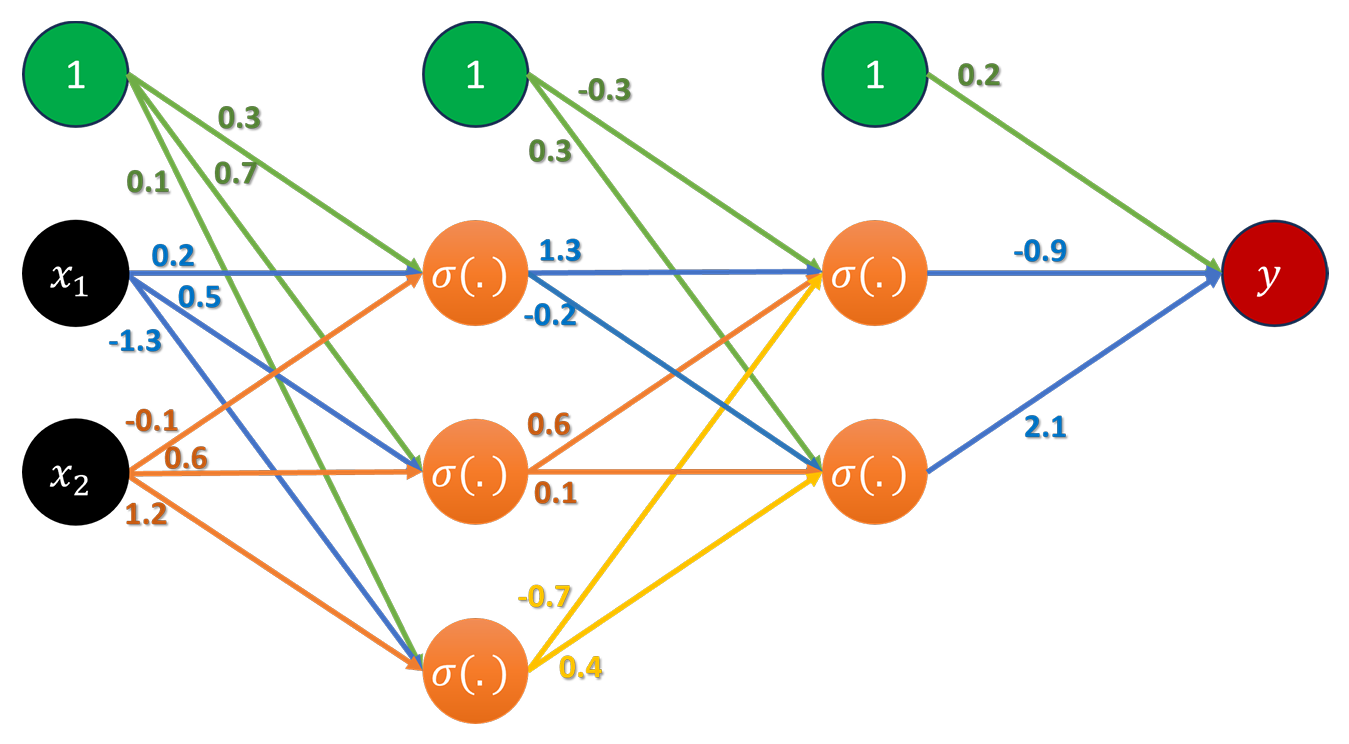
\includegraphics[height=3.0cm, keepaspectratio]{images/figura_1.png}
    \caption{Arquitectura de la red neuronal $f: \mathbb{R}^2 \to \mathbb{R}$. Nodos negros: entradas $x_1, x_2$; nodos verdes: sesgos unitarios; nodos naranjas: capas ocultas con activación sigmoide $\sigma$; nodo rojo: salida lineal $y = f_2$.}
    \label{fig:red}
\end{figure}

Para analizar el funcionamiento del algoritmo de retropropagación, trabajamos con la red neuronal que se muestra en la Figura~\ref{fig:red}. Esta red toma una entrada de dos dimensiones $\mathbf{x} = [x_1, x_2]^T$, tiene dos capas ocultas, con 3 neuronas en la primera y 2 en la segunda, que aplican la función de activación sigmoide $\sigma(t) = \frac{1}{1 + e^{-t}}$, y finalmente genera un valor de salida $f_2$ combinando las señales de forma lineal.

Mirando las conexiones del diagrama, extraemos los valores iniciales de los pesos y los sesgos para cada capa:
\begin{itemize}
    \item \textbf{Capa 0, primera capa oculta con 3 neuronas:}
    \[
    \boldsymbol{\beta}_0 = \begin{bmatrix} 0.3 \\ 0.7 \\ 0.1 \end{bmatrix}, \quad
    \boldsymbol{\Omega}_0 = \begin{bmatrix} 0.2 & -0.1 \\ 0.5 & 0.6 \\ -1.3 & 1.2 \end{bmatrix}
    \]
    \item \textbf{Capa 1, segunda capa oculta con 2 neuronas:}
    \[
    \boldsymbol{\beta}_1 = \begin{bmatrix} -0.3 \\ 0.3 \end{bmatrix}, \quad
    \boldsymbol{\Omega}_1 = \begin{bmatrix} 1.3 & 0.6 & -0.7 \\ -0.2 & 0.1 & 0.4 \end{bmatrix}
    \]
    \item \textbf{Capa 2, capa de salida lineal con 1 neurona:}
    \[
    \boldsymbol{\beta}_2 = [0.2], \quad
    \boldsymbol{\Omega}_2 = \begin{bmatrix} -0.9 & 2.1 \end{bmatrix}
    \]
\end{itemize}

Para el entrenamiento usamos estos tres datos:
\[
(\mathbf{x}^{(1)}, y^{(1)}) = \left(\begin{bmatrix} 1 \\ 1 \end{bmatrix}, 1\right), \quad
(\mathbf{x}^{(2)}, y^{(2)}) = \left(\begin{bmatrix} 0 \\ 2 \end{bmatrix}, 1\right), \quad
(\mathbf{x}^{(3)}, y^{(3)}) = \left(\begin{bmatrix} -1 \\ 1 \end{bmatrix}, 0\right)
\]
Para medir el error de la red usamos la función de pérdida cuadrática. Calculamos el error de cada dato por separado como $\ell_i = (f_2(\mathbf{x}_i) - y_i)^2$, y obtenemos la pérdida total del \textit{batch} promediando los tres errores: $L = \frac{1}{3} \sum_{i=1}^3 \ell_i$.

\clearpage
\subsection*{Formulación del paso hacia adelante}

Siguiendo la formulación del libro (ecuación 7.24), el cálculo hacia adelante para la red del enunciado se escribe así:
\begin{gather}
    \mathbf{f}_0 = \boldsymbol{\beta}_0 + \boldsymbol{\Omega}_0 \mathbf{x}_i \\
    \mathbf{h}_k = \sigma(\mathbf{f}_{k-1}), \quad k \in \{1, 2\} \\
    \mathbf{f}_k = \boldsymbol{\beta}_k + \boldsymbol{\Omega}_k \mathbf{h}_k, \quad k \in \{1, 2\}
\end{gather}
En estas ecuaciones, cada término tiene una dimensión y un rol bien definidos:
\begin{itemize}
    \item $\mathbf{x}_i \in \mathbb{R}^{2 \times 1}$: vector con los dos datos de entrada, correspondientes a los nodos negros del diagrama.
    \item $\boldsymbol{\beta}_0 \in \mathbb{R}^{3 \times 1}, \; \boldsymbol{\beta}_1 \in \mathbb{R}^{2 \times 1}$: vectores de sesgo de las capas ocultas, y $\beta_2 \in \mathbb{R}$ sesgo escalar de la salida, correspondiente a los nodos verdes del diagrama.
    \item $\boldsymbol{\Omega}_0 \in \mathbb{R}^{3 \times 2}, \; \boldsymbol{\Omega}_1 \in \mathbb{R}^{2 \times 3}, \; \boldsymbol{\Omega}_2 \in \mathbb{R}^{1 \times 2}$: matrices de pesos que multiplican a las entradas de cada capa, donde las filas corresponden a las neuronas de destino y las columnas a las neuronas de origen.
    \item $\mathbf{f}_0 \in \mathbb{R}^{3 \times 1}, \; \mathbf{f}_1 \in \mathbb{R}^{2 \times 1}$: preactivaciones o sumas ponderadas antes de aplicar la función de activación en las capas ocultas.
    \item $\mathbf{h}_1 \in \mathbb{R}^{3 \times 1}, \; \mathbf{h}_2 \in \mathbb{R}^{2 \times 1}$: activaciones de las capas ocultas tras evaluar la sigmoide, mostradas en color naranja.
    \item $f_2 \in \mathbb{R}$: predicción escalar final calculada por la red en el nodo rojo de salida.
\end{itemize}

\subsection*{Adaptación del paso hacia atrás para activación sigmoide}

En el libro (ecuación 7.25) se formula la retropropagación para activación ReLU. Como la red del enunciado utiliza activación sigmoide $\sigma(t) = \frac{1}{1 + e^{-t}}$, adaptamos las ecuaciones calculando primero su derivada analítica:
\[
\frac{d\sigma(t)}{dt} = \frac{e^{-t}}{(1 + e^{-t})^2} = \left(\frac{1}{1 + e^{-t}}\right)\left(1 - \frac{1}{1 + e^{-t}}\right) = \sigma(t)(1 - \sigma(t))
\]
Aplicando la regla de la cadena, el gradiente de la pérdida se transmite hacia la capa anterior multiplicando por los pesos traspuestos y por la derivada de la sigmoide en cada neurona:
\[
\frac{\partial \ell_i}{\partial \mathbf{f}_{k-1}} = \Big( \sigma(\mathbf{f}_{k-1}) \odot (\mathbf{1} - \sigma(\mathbf{f}_{k-1})) \Big) \odot \left( \boldsymbol{\Omega}_k^T \frac{\partial \ell_i}{\partial \mathbf{f}_k} \right)
\]
donde el símbolo $\odot$ representa el producto de Hadamard, es decir, la multiplicación elemento a elemento. De este modo, las ecuaciones completas de retropropagación para la red quedan de la siguiente forma:
\begin{gather}
    \frac{\partial \ell_i}{\partial \boldsymbol{\beta}_k} = \frac{\partial \ell_i}{\partial \mathbf{f}_k}, \quad k \in \{2, 1, 0\} \\
    \frac{\partial \ell_i}{\partial \boldsymbol{\Omega}_k} = \frac{\partial \ell_i}{\partial \mathbf{f}_k} \mathbf{h}_k^T, \quad k \in \{2, 1, 0\}, \quad \text{donde } \mathbf{h}_0 = \mathbf{x}_i \\
    \frac{\partial \ell_i}{\partial \mathbf{f}_{k-1}} = \Big[ \sigma(\mathbf{f}_{k-1}) \odot (\mathbf{1} - \sigma(\mathbf{f}_{k-1})) \Big] \odot \left( \boldsymbol{\Omega}_k^T \frac{\partial \ell_i}{\partial \mathbf{f}_k} \right), \quad k \in \{2, 1\}
\end{gather}

Las dimensiones de los componentes en este paso hacia atrás son:
\begin{itemize}
    \item $\frac{\partial \ell_i}{\partial f_2} \in \mathbb{R}$: derivada escalar del error cuadrático respecto a la salida, calculada como $2(f_2 - y_i)$.
    \item $\frac{\partial \ell_i}{\partial \beta_2} \in \mathbb{R}, \; \frac{\partial \ell_i}{\partial \boldsymbol{\beta}_1} \in \mathbb{R}^{2 \times 1}, \; \frac{\partial \ell_i}{\partial \boldsymbol{\beta}_0} \in \mathbb{R}^{3 \times 1}$: gradientes respecto a los sesgos de cada capa, iguales a $\frac{\partial \ell_i}{\partial \mathbf{f}_k}$.
    \item $\frac{\partial \ell_i}{\partial \boldsymbol{\Omega}_2} \in \mathbb{R}^{1 \times 2}, \; \frac{\partial \ell_i}{\partial \boldsymbol{\Omega}_1} \in \mathbb{R}^{2 \times 3}, \; \frac{\partial \ell_i}{\partial \boldsymbol{\Omega}_0} \in \mathbb{R}^{3 \times 2}$: gradientes matriciales respecto a los pesos, obtenidos por el producto exterior $\frac{\partial \ell_i}{\partial \mathbf{f}_k} \mathbf{h}_k^T$.
    \item $\frac{\partial \ell_i}{\partial \mathbf{f}_1} \in \mathbb{R}^{2 \times 1}, \; \frac{\partial \ell_i}{\partial \mathbf{f}_0} \in \mathbb{R}^{3 \times 1}$: gradientes respecto a las preactivaciones de las capas ocultas.
    \item $\boldsymbol{\Omega}_k^T \frac{\partial \ell_i}{\partial \mathbf{f}_k}$: proyección del gradiente desde la capa siguiente hacia la capa previa.
    \item $\sigma(\mathbf{f}_{k-1}) \odot (\mathbf{1} - \sigma(\mathbf{f}_{k-1})) \in \mathbb{R}^{D_{k-1} \times 1}$: derivada local de la función sigmoide en cada neurona.
    \item $\odot$: multiplicación elemento a elemento, o producto de Hadamard.
\end{itemize}

\subsection*{Cálculo explícito del paso de optimización sobre el batch}

\subsubsection*{Dato 1: $\mathbf{x}^{(1)} = [1, 1]^T, \quad y^{(1)} = 1$}

\paragraph{Paso hacia adelante:}
\begin{itemize}
    \item \textbf{Capa 0: preactivación y activación}
    \begin{align*}
    \mathbf{f}_0^{(1)} &= \boldsymbol{\beta}_0 + \boldsymbol{\Omega}_0 \mathbf{x}^{(1)} = \begin{bmatrix} 0.3 \\ 0.7 \\ 0.1 \end{bmatrix} + \begin{bmatrix} 0.2 & -0.1 \\ 0.5 & 0.6 \\ -1.3 & 1.2 \end{bmatrix} \begin{bmatrix} 1 \\ 1 \end{bmatrix} = \begin{bmatrix} 0.4 \\ 1.8 \\ 0.0 \end{bmatrix} \\[0.1cm]
    \mathbf{h}_1^{(1)} &= \sigma(\mathbf{f}_0^{(1)}) = \begin{bmatrix} \sigma(0.4) \\ \sigma(1.8) \\ \sigma(0.0) \end{bmatrix} = \begin{bmatrix} \frac{1}{1+e^{-0.4}} \\ \frac{1}{1+e^{-1.8}} \\ \frac{1}{1+e^0} \end{bmatrix} = \begin{bmatrix} 0.5987 \\ 0.8581 \\ 0.5000 \end{bmatrix}
    \end{align*}

    \item \textbf{Capa 1: preactivación y activación}
    \begin{align*}
    \mathbf{f}_1^{(1)} &= \boldsymbol{\beta}_1 + \boldsymbol{\Omega}_1 \mathbf{h}_1^{(1)} = \begin{bmatrix} -0.3 \\ 0.3 \end{bmatrix} + \begin{bmatrix} 1.3 & 0.6 & -0.7 \\ -0.2 & 0.1 & 0.4 \end{bmatrix} \begin{bmatrix} 0.5987 \\ 0.8581 \\ 0.5000 \end{bmatrix} = \begin{bmatrix} 0.6432 \\ 0.4661 \end{bmatrix} \\[0.1cm]
    \mathbf{h}_2^{(1)} &= \sigma(\mathbf{f}_1^{(1)}) = \begin{bmatrix} \sigma(0.6432) \\ \sigma(0.4661) \end{bmatrix} = \begin{bmatrix} 0.6555 \\ 0.6145 \end{bmatrix}
    \end{align*}

    \item \textbf{Capa 2: salida y cálculo de pérdida}
    \begin{align*}
    f_2^{(1)} &= \beta_2 + \boldsymbol{\Omega}_2 \mathbf{h}_2^{(1)} = 0.2 + \begin{bmatrix} -0.9 & 2.1 \end{bmatrix} \begin{bmatrix} 0.6555 \\ 0.6145 \end{bmatrix} = 0.9004 \\[0.1cm]
    \ell_1 &= (f_2^{(1)} - y^{(1)})^2 = (0.9004 - 1)^2 = (-0.09956)^2 = \mathbf{0.009914}
    \end{align*}
\end{itemize}

\paragraph{Paso hacia atrás:}
\begin{itemize}
    \item \textbf{Capa 2: gradientes de la salida}
    \begin{align*}
    \frac{\partial \ell_1}{\partial f_2} &= 2(f_2^{(1)} - y^{(1)}) = 2(0.9004 - 1) = -0.19914 \implies \frac{\partial \ell_1}{\partial \beta_2} = \mathbf{-0.19914} \\[0.1cm]
    \frac{\partial \ell_1}{\partial \boldsymbol{\Omega}_2} &= \frac{\partial \ell_1}{\partial f_2} (\mathbf{h}_2^{(1)})^T = -0.19914 \begin{bmatrix} 0.6555 & 0.6145 \end{bmatrix} = \mathbf{\begin{bmatrix} -0.13053 & -0.12236 \end{bmatrix}}
    \end{align*}

    \item \textbf{Capa 1: gradientes de la segunda capa oculta}
    \begin{align*}
    \frac{\partial \ell_1}{\partial \mathbf{f}_1} &= \big[ \mathbf{h}_2^{(1)} \odot (\mathbf{1} - \mathbf{h}_2^{(1)}) \big] \odot \left( \boldsymbol{\Omega}_2^T \frac{\partial \ell_1}{\partial f_2} \right) = \begin{bmatrix} 0.22582 \\ 0.23690 \end{bmatrix} \odot \begin{bmatrix} 0.17923 \\ -0.41819 \end{bmatrix} = \mathbf{\begin{bmatrix} 0.04047 \\ -0.09907 \end{bmatrix}} = \frac{\partial \ell_1}{\partial \boldsymbol{\beta}_1} \\[0.1cm]
    \frac{\partial \ell_1}{\partial \boldsymbol{\Omega}_1} &= \frac{\partial \ell_1}{\partial \mathbf{f}_1} (\mathbf{h}_1^{(1)})^T = \begin{bmatrix} 0.04047 \\ -0.09907 \end{bmatrix} \begin{bmatrix} 0.5987 & 0.8581 & 0.5000 \end{bmatrix} = \mathbf{\begin{bmatrix} 0.02423 & 0.03473 & 0.02024 \\ -0.05931 & -0.08502 & -0.04954 \end{bmatrix}}
    \end{align*}

    \item \textbf{Capa 0: gradientes de la primera capa oculta}
    \begin{align*}
    \frac{\partial \ell_1}{\partial \mathbf{f}_0} &= \big[ \mathbf{h}_1^{(1)} \odot (\mathbf{1} - \mathbf{h}_1^{(1)}) \big] \odot \left( \boldsymbol{\Omega}_1^T \frac{\partial \ell_1}{\partial \mathbf{f}_1} \right) = \begin{bmatrix} 0.24026 \\ 0.12176 \\ 0.25000 \end{bmatrix} \odot \begin{bmatrix} 0.07242 \\ 0.01437 \\ -0.06796 \end{bmatrix} = \mathbf{\begin{bmatrix} 0.01740 \\ 0.00175 \\ -0.01699 \end{bmatrix}} = \frac{\partial \ell_1}{\partial \boldsymbol{\beta}_0} \\[0.1cm]
    \frac{\partial \ell_1}{\partial \boldsymbol{\Omega}_0} &= \frac{\partial \ell_1}{\partial \mathbf{f}_0} (\mathbf{x}^{(1)})^T = \begin{bmatrix} 0.01740 \\ 0.00175 \\ -0.01699 \end{bmatrix} \begin{bmatrix} 1 & 1 \end{bmatrix} = \mathbf{\begin{bmatrix} 0.01740 & 0.01740 \\ 0.00175 & 0.00175 \\ -0.01699 & -0.01699 \end{bmatrix}}
    \end{align*}
\end{itemize}

\subsubsection*{Dato 2: $\mathbf{x}^{(2)} = [0, 2]^T, \quad y^{(2)} = 1$}

\paragraph{Paso hacia adelante:}
\begin{itemize}
    \item \textbf{Capa 0: preactivación y activación}
    \begin{align*}
    \mathbf{f}_0^{(2)} &= \boldsymbol{\beta}_0 + \boldsymbol{\Omega}_0 \mathbf{x}^{(2)} = \begin{bmatrix} 0.3 \\ 0.7 \\ 0.1 \end{bmatrix} + \begin{bmatrix} 0.2 & -0.1 \\ 0.5 & 0.6 \\ -1.3 & 1.2 \end{bmatrix} \begin{bmatrix} 0 \\ 2 \end{bmatrix} = \begin{bmatrix} 0.1 \\ 1.9 \\ 2.5 \end{bmatrix} \\[0.1cm]
    \mathbf{h}_1^{(2)} &= \sigma(\mathbf{f}_0^{(2)}) = \begin{bmatrix} \sigma(0.1) \\ \sigma(1.9) \\ \sigma(2.5) \end{bmatrix} = \begin{bmatrix} 0.5250 \\ 0.8699 \\ 0.9241 \end{bmatrix}
    \end{align*}

    \item \textbf{Capa 1: preactivación y activación}
    \begin{align*}
    \mathbf{f}_1^{(2)} &= \boldsymbol{\beta}_1 + \boldsymbol{\Omega}_1 \mathbf{h}_1^{(2)} = \begin{bmatrix} -0.3 \\ 0.3 \end{bmatrix} + \begin{bmatrix} 1.3 & 0.6 & -0.7 \\ -0.2 & 0.1 & 0.4 \end{bmatrix} \begin{bmatrix} 0.5250 \\ 0.8699 \\ 0.9241 \end{bmatrix} = \begin{bmatrix} 0.2575 \\ 0.6517 \end{bmatrix} \\[0.1cm]
    \mathbf{h}_2^{(2)} &= \sigma(\mathbf{f}_1^{(2)}) = \begin{bmatrix} 0.5640 \\ 0.6574 \end{bmatrix}
    \end{align*}

    \item \textbf{Capa 2: salida y cálculo de pérdida}
    \begin{align*}
    f_2^{(2)} &= \beta_2 + \boldsymbol{\Omega}_2 \mathbf{h}_2^{(2)} = 0.2 + \begin{bmatrix} -0.9 & 2.1 \end{bmatrix} \begin{bmatrix} 0.5640 \\ 0.6574 \end{bmatrix} = 1.0729 \\[0.1cm]
    \ell_2 &= (1.0729 - 1)^2 = \mathbf{0.005312}
    \end{align*}
\end{itemize}

\paragraph{Paso hacia atrás:}
\begin{itemize}
    \item \textbf{Capa 2: gradientes de la salida}
    \begin{align*}
    \frac{\partial \ell_2}{\partial f_2} &= 2(1.0729 - 1) = 0.14576 \implies \frac{\partial \ell_2}{\partial \beta_2} = \mathbf{0.14576} \\[0.1cm]
    \frac{\partial \ell_2}{\partial \boldsymbol{\Omega}_2} &= \frac{\partial \ell_2}{\partial f_2} (\mathbf{h}_2^{(2)})^T = 0.14576 \begin{bmatrix} 0.5640 & 0.6574 \end{bmatrix} = \mathbf{\begin{bmatrix} 0.08221 & 0.09582 \end{bmatrix}}
    \end{align*}

    \item \textbf{Capa 1: gradientes de la segunda capa oculta}
    \begin{align*}
    \frac{\partial \ell_2}{\partial \mathbf{f}_1} &= \big[\mathbf{h}_2^{(2)} \odot (\mathbf{1} - \mathbf{h}_2^{(2)})\big] \odot \left(\boldsymbol{\Omega}_2^T \frac{\partial \ell_2}{\partial f_2}\right) = \begin{bmatrix} 0.24590 \\ 0.22522 \end{bmatrix} \odot \begin{bmatrix} -0.13118 \\ 0.30610 \end{bmatrix} = \mathbf{\begin{bmatrix} -0.03226 \\ 0.06894 \end{bmatrix}} = \frac{\partial \ell_2}{\partial \boldsymbol{\beta}_1} \\[0.1cm]
    \frac{\partial \ell_2}{\partial \boldsymbol{\Omega}_1} &= \frac{\partial \ell_2}{\partial \mathbf{f}_1} (\mathbf{h}_1^{(2)})^T = \mathbf{\begin{bmatrix} -0.01694 & -0.02806 & -0.02981 \\ 0.03619 & 0.05997 & 0.06371 \end{bmatrix}}
    \end{align*}

    \item \textbf{Capa 0: gradientes de la primera capa oculta}
    \begin{align*}
    \frac{\partial \ell_2}{\partial \mathbf{f}_0} &= \big[\mathbf{h}_1^{(2)} \odot (\mathbf{1} - \mathbf{h}_1^{(2)})\big] \odot \left(\boldsymbol{\Omega}_1^T \frac{\partial \ell_2}{\partial \mathbf{f}_1}\right) = \begin{bmatrix} 0.24938 \\ 0.11317 \\ 0.07014 \end{bmatrix} \odot \begin{bmatrix} -0.05573 \\ -0.01246 \\ 0.05016 \end{bmatrix} = \mathbf{\begin{bmatrix} -0.01390 \\ -0.00141 \\ 0.00352 \end{bmatrix}} = \frac{\partial \ell_2}{\partial \boldsymbol{\beta}_0} \\[0.1cm]
    \frac{\partial \ell_2}{\partial \boldsymbol{\Omega}_0} &= \frac{\partial \ell_2}{\partial \mathbf{f}_0} (\mathbf{x}^{(2)})^T = \mathbf{\begin{bmatrix} 0 & -0.02779 \\ 0 & -0.00282 \\ 0 & 0.00703 \end{bmatrix}}
    \end{align*}
\end{itemize}

\subsubsection*{Dato 3: $\mathbf{x}^{(3)} = [-1, 1]^T, \quad y^{(3)} = 0$}

\paragraph{Paso hacia adelante:}
\begin{itemize}
    \item \textbf{Capa 0: preactivación y activación}
    \begin{align*}
    \mathbf{f}_0^{(3)} &= \boldsymbol{\beta}_0 + \boldsymbol{\Omega}_0 \mathbf{x}^{(3)} = \begin{bmatrix} 0.3 \\ 0.7 \\ 0.1 \end{bmatrix} + \begin{bmatrix} 0.2 & -0.1 \\ 0.5 & 0.6 \\ -1.3 & 1.2 \end{bmatrix} \begin{bmatrix} -1 \\ 1 \end{bmatrix} = \begin{bmatrix} 0.0 \\ 0.8 \\ 2.6 \end{bmatrix} \\[0.1cm]
    \mathbf{h}_1^{(3)} &= \sigma(\mathbf{f}_0^{(3)}) = \begin{bmatrix} \sigma(0.0) \\ \sigma(0.8) \\ \sigma(2.6) \end{bmatrix} = \begin{bmatrix} 0.5000 \\ 0.6900 \\ 0.9309 \end{bmatrix}
    \end{align*}

    \item \textbf{Capa 1: preactivación y activación}
    \begin{align*}
    \mathbf{f}_1^{(3)} &= \boldsymbol{\beta}_1 + \boldsymbol{\Omega}_1 \mathbf{h}_1^{(3)} = \begin{bmatrix} -0.3 \\ 0.3 \end{bmatrix} + \begin{bmatrix} 1.3 & 0.6 & -0.7 \\ -0.2 & 0.1 & 0.4 \end{bmatrix} \begin{bmatrix} 0.5000 \\ 0.6900 \\ 0.9309 \end{bmatrix} = \begin{bmatrix} 0.1124 \\ 0.6413 \end{bmatrix} \\[0.1cm]
    \mathbf{h}_2^{(3)} &= \sigma(\mathbf{f}_1^{(3)}) = \begin{bmatrix} 0.5281 \\ 0.6551 \end{bmatrix}
    \end{align*}

    \item \textbf{Capa 2: salida y cálculo de pérdida}
    \begin{align*}
    f_2^{(3)} &= \beta_2 + \boldsymbol{\Omega}_2 \mathbf{h}_2^{(3)} = 0.2 + \begin{bmatrix} -0.9 & 2.1 \end{bmatrix} \begin{bmatrix} 0.5281 \\ 0.6551 \end{bmatrix} = 1.1004 \\[0.1cm]
    \ell_3 &= (1.1004 - 0)^2 = \mathbf{1.210792}
    \end{align*}
\end{itemize}

\paragraph{Paso hacia atrás:}
\begin{itemize}
    \item \textbf{Capa 2: gradientes de la salida}
    \begin{align*}
    \frac{\partial \ell_3}{\partial f_2} &= 2(1.1004 - 0) = 2.20072 \implies \frac{\partial \ell_3}{\partial \beta_2} = \mathbf{2.20072} \\[0.1cm]
    \frac{\partial \ell_3}{\partial \boldsymbol{\Omega}_2} &= \frac{\partial \ell_3}{\partial f_2} (\mathbf{h}_2^{(3)})^T = 2.20072 \begin{bmatrix} 0.5281 & 0.6551 \end{bmatrix} = \mathbf{\begin{bmatrix} 1.16213 & 1.44160 \end{bmatrix}}
    \end{align*}

    \item \textbf{Capa 1: gradientes de la segunda capa oculta}
    \begin{align*}
    \frac{\partial \ell_3}{\partial \mathbf{f}_1} &= \big[\mathbf{h}_2^{(3)} \odot (\mathbf{1} - \mathbf{h}_2^{(3)})\big] \odot \left(\boldsymbol{\Omega}_2^T \frac{\partial \ell_3}{\partial f_2}\right) = \begin{bmatrix} 0.24921 \\ 0.22594 \end{bmatrix} \odot \begin{bmatrix} -1.98065 \\ 4.62151 \end{bmatrix} = \mathbf{\begin{bmatrix} -0.49360 \\ 1.04426 \end{bmatrix}} = \frac{\partial \ell_3}{\partial \boldsymbol{\beta}_1} \\[0.1cm]
    \frac{\partial \ell_3}{\partial \boldsymbol{\Omega}_1} &= \frac{\partial \ell_3}{\partial \mathbf{f}_1} (\mathbf{h}_1^{(3)})^T = \mathbf{\begin{bmatrix} -0.24680 & -0.34057 & -0.45947 \\ 0.52213 & 0.72052 & 0.97207 \end{bmatrix}}
    \end{align*}

    \item \textbf{Capa 0: gradientes de la primera capa oculta}
    \begin{align*}
    \frac{\partial \ell_3}{\partial \mathbf{f}_0} &= \big[\mathbf{h}_1^{(3)} \odot (\mathbf{1} - \mathbf{h}_1^{(3)})\big] \odot \left(\boldsymbol{\Omega}_1^T \frac{\partial \ell_3}{\partial \mathbf{f}_1}\right) = \begin{bmatrix} 0.25000 \\ 0.21390 \\ 0.06433 \end{bmatrix} \odot \begin{bmatrix} -0.85053 \\ -0.19173 \\ 0.76322 \end{bmatrix} = \mathbf{\begin{bmatrix} -0.21263 \\ -0.04101 \\ 0.04912 \end{bmatrix}} = \frac{\partial \ell_3}{\partial \boldsymbol{\beta}_0} \\[0.1cm]
    \frac{\partial \ell_3}{\partial \boldsymbol{\Omega}_0} &= \frac{\partial \ell_3}{\partial \mathbf{f}_0} (\mathbf{x}^{(3)})^T = \mathbf{\begin{bmatrix} 0.21263 & -0.21263 \\ 0.04101 & -0.04101 \\ -0.04912 & 0.04912 \end{bmatrix}}
    \end{align*}
\end{itemize}

\subsubsection*{Promedio del batch y actualización con $\alpha = 1.0$}

Con los gradientes calculados para los tres datos, sacamos el promedio exacto para saber en qué dirección ajustar los parámetros:
\[
\nabla_{\boldsymbol{\theta}} L = \frac{1}{3} \sum_{i=1}^3 \nabla_{\boldsymbol{\theta}} \ell_i = \frac{1}{3} \Big( \underbrace{\nabla_{\boldsymbol{\theta}} \ell_1}_{\text{Dato 1}} + \underbrace{\nabla_{\boldsymbol{\theta}} \ell_2}_{\text{Dato 2}} + \underbrace{\nabla_{\boldsymbol{\theta}} \ell_3}_{\text{Dato 3}} \Big)
\]
Sumamos los términos de los tres datos y dividimos entre 3 para cada componente:
\begin{align*}
\frac{\partial L}{\partial \boldsymbol{\beta}_2} &= \frac{1}{3}\left( \underbrace{[-0.19914]}_{\text{Dato 1}} + \underbrace{[0.14576]}_{\text{Dato 2}} + \underbrace{[2.20072]}_{\text{Dato 3}} \right) = \frac{[2.14734]}{3} = \mathbf{[0.71578]} \\[0.2cm]
\frac{\partial L}{\partial \boldsymbol{\Omega}_2} &= \frac{1}{3}\left( \underbrace{[-0.13053, \; -0.12236]}_{\text{Dato 1}} + \underbrace{[0.08221, \; 0.09582]}_{\text{Dato 2}} + \underbrace{[1.16213, \; 1.44160]}_{\text{Dato 3}} \right) = \mathbf{\begin{bmatrix} 0.37127 & 0.47169 \end{bmatrix}} \\[0.2cm]
\frac{\partial L}{\partial \boldsymbol{\beta}_1} &= \frac{1}{3}\left( \underbrace{\begin{bmatrix} 0.04047 \\ -0.09907 \end{bmatrix}}_{\text{Dato 1}} + \underbrace{\begin{bmatrix} -0.03226 \\ 0.06894 \end{bmatrix}}_{\text{Dato 2}} + \underbrace{\begin{bmatrix} -0.49360 \\ 1.04426 \end{bmatrix}}_{\text{Dato 3}} \right) = \mathbf{\begin{bmatrix} -0.16180 \\ 0.33805 \end{bmatrix}} \\[0.2cm]
\frac{\partial L}{\partial \boldsymbol{\Omega}_1} &= \frac{1}{3}\Bigg( \underbrace{\begin{bmatrix} 0.02423 & 0.03473 & 0.02024 \\ -0.05931 & -0.08502 & -0.04954 \end{bmatrix}}_{\text{Dato 1}} + \underbrace{\begin{bmatrix} -0.01694 & -0.02806 & -0.02981 \\ 0.03619 & 0.05997 & 0.06371 \end{bmatrix}}_{\text{Dato 2}} \\
&\hspace{1cm} + \underbrace{\begin{bmatrix} -0.24680 & -0.34057 & -0.45947 \\ 0.52213 & 0.72052 & 0.97207 \end{bmatrix}}_{\text{Dato 3}} \Bigg) = \mathbf{\begin{bmatrix} -0.07983 & -0.11130 & -0.15635 \\ 0.16634 & 0.23182 & 0.32875 \end{bmatrix}} \\[0.2cm]
\frac{\partial L}{\partial \boldsymbol{\beta}_0} &= \frac{1}{3}\left( \underbrace{\begin{bmatrix} 0.01740 \\ 0.00175 \\ -0.01699 \end{bmatrix}}_{\text{Dato 1}} + \underbrace{\begin{bmatrix} -0.01390 \\ -0.00141 \\ 0.00352 \end{bmatrix}}_{\text{Dato 2}} + \underbrace{\begin{bmatrix} -0.21263 \\ -0.04101 \\ 0.04912 \end{bmatrix}}_{\text{Dato 3}} \right) = \mathbf{\begin{bmatrix} -0.06971 \\ -0.01356 \\ 0.01188 \end{bmatrix}} \\[0.2cm]
\frac{\partial L}{\partial \boldsymbol{\Omega}_0} &= \frac{1}{3}\Bigg( \underbrace{\begin{bmatrix} 0.01740 & 0.01740 \\ 0.00175 & 0.00175 \\ -0.01699 & -0.01699 \end{bmatrix}}_{\text{Dato 1}} + \underbrace{\begin{bmatrix} 0 & -0.02779 \\ 0 & -0.00282 \\ 0 & 0.00703 \end{bmatrix}}_{\text{Dato 2}} + \underbrace{\begin{bmatrix} 0.21263 & -0.21263 \\ 0.04101 & -0.04101 \\ -0.04912 & 0.04912 \end{bmatrix}}_{\text{Dato 3}} \Bigg) \\
&= \mathbf{\begin{bmatrix} 0.07668 & -0.07434 \\ 0.01425 & -0.01403 \\ -0.02204 & 0.01305 \end{bmatrix}}
\end{align*}

Con la tasa de aprendizaje $\alpha = 1.0$, actualizamos los parámetros restando este gradiente promedio a los valores anteriores ($\boldsymbol{\theta}^{(t+1)} = \boldsymbol{\theta}^{(t)} - 1.0 \cdot \nabla_{\boldsymbol{\theta}} L$):

\begin{align*}
\boldsymbol{\beta}_0^{\text{nuevo}} &= \begin{bmatrix} 0.3 \\ 0.7 \\ 0.1 \end{bmatrix} - 1.0 \begin{bmatrix} -0.06971 \\ -0.01356 \\ 0.01188 \end{bmatrix} = \mathbf{\begin{bmatrix} 0.36971 \\ 0.71356 \\ 0.08812 \end{bmatrix}} \\[0.2cm]
\boldsymbol{\Omega}_0^{\text{nuevo}} &= \begin{bmatrix} 0.2 & -0.1 \\ 0.5 & 0.6 \\ -1.3 & 1.2 \end{bmatrix} - 1.0 \begin{bmatrix} 0.07668 & -0.07434 \\ 0.01425 & -0.01403 \\ -0.02204 & 0.01305 \end{bmatrix} = \mathbf{\begin{bmatrix} 0.12332 & -0.02566 \\ 0.48575 & 0.61403 \\ -1.27796 & 1.18695 \end{bmatrix}} \\[0.2cm]
\boldsymbol{\beta}_1^{\text{nuevo}} &= \begin{bmatrix} -0.3 \\ 0.3 \end{bmatrix} - 1.0 \begin{bmatrix} -0.16180 \\ 0.33805 \end{bmatrix} = \mathbf{\begin{bmatrix} -0.13820 \\ -0.03805 \end{bmatrix}} \\[0.2cm]
\boldsymbol{\Omega}_1^{\text{nuevo}} &= \begin{bmatrix} 1.3 & 0.6 & -0.7 \\ -0.2 & 0.1 & 0.4 \end{bmatrix} - 1.0 \begin{bmatrix} -0.07983 & -0.11130 & -0.15635 \\ 0.16634 & 0.23182 & 0.32875 \end{bmatrix} = \mathbf{\begin{bmatrix} 1.37983 & 0.71130 & -0.54365 \\ -0.36634 & -0.13182 & 0.07125 \end{bmatrix}} \\[0.2cm]
\boldsymbol{\beta}_2^{\text{nuevo}} &= [0.2] - 1.0 [0.71578] = \mathbf{[-0.51578]} \\[0.2cm]
\boldsymbol{\Omega}_2^{\text{nuevo}} &= \begin{bmatrix} -0.9 & 2.1 \end{bmatrix} - 1.0 \begin{bmatrix} 0.37127 & 0.47169 \end{bmatrix} = \mathbf{\begin{bmatrix} -1.27127 & 1.62831 \end{bmatrix}}
\end{align*}

Como detalle adicional, la pérdida inicial promedio de los tres datos fue $L^{(0)} = \frac{0.009914 + 0.005312 + 1.210792}{3} \approx 0.4087$. Al aplicar este primer paso con $\alpha = 1.0$, el avance es bastante grande para los valores que maneja la red y hace que la salida se pase de largo (\textit{overshooting}). En la práctica, si usamos una tasa más pequeña y habitual como $\alpha \le 0.2$, el error va bajando de forma constante paso a paso.



\subsection*{Verificación computacional y práctica en el Notebook 7.2}

Para comprobar que los cálculos que hicimos a mano coinciden con la simulación en máquina, programamos la arquitectura completa de la Figura~\ref{fig:red} en el Notebook 7.2 vectorizando el paso hacia adelante y el paso hacia atrás.

Para revisar la exactitud de las derivadas, se implementó una comprobación numérica por diferencias finitas con una perturbación de $\epsilon = 10^{-6}$:
\[
\frac{\partial L}{\partial \theta_j} \approx \frac{L(\boldsymbol{\theta} + \epsilon \mathbf{e}_j) - L(\boldsymbol{\theta} - \epsilon \mathbf{e}_j)}{2\epsilon}
\]
Al contrastar las derivadas analíticas con las numéricas en los 20 parámetros de la red, correspondientes a $\boldsymbol{\Omega}_0$ con 6 pesos, $\boldsymbol{\beta}_0$ con 3 sesgos, $\boldsymbol{\Omega}_1$ con 6 pesos, $\boldsymbol{\beta}_1$ con 2 sesgos, $\boldsymbol{\Omega}_2$ con 2 pesos y $\beta_2$ con 1 sesgo, la diferencia fue menor a $10^{-7}$, lo que confirma con exactitud cada matriz y vector que obtuvimos. Además, al probar una tasa de aprendizaje moderada de $\alpha = 0.2$, el error disminuye de forma constante desde $0.4087$ hasta $0.2798$, confirmando que los gradientes apuntan en la dirección de descenso correcta hacia el mínimo.


\section*{II-B. Algoritmos de optimización}

Para entender cómo se comportan los optimizadores al entrenar una red neuronal, usamos la superficie del enunciado como función objetivo:
\[
f(x, y) = \frac{\sin\left(0.8(x^2 + y^2)\right)}{(x^2 + y^2)^{0.9}}
\]

\begin{figure}[H]
    \centering
    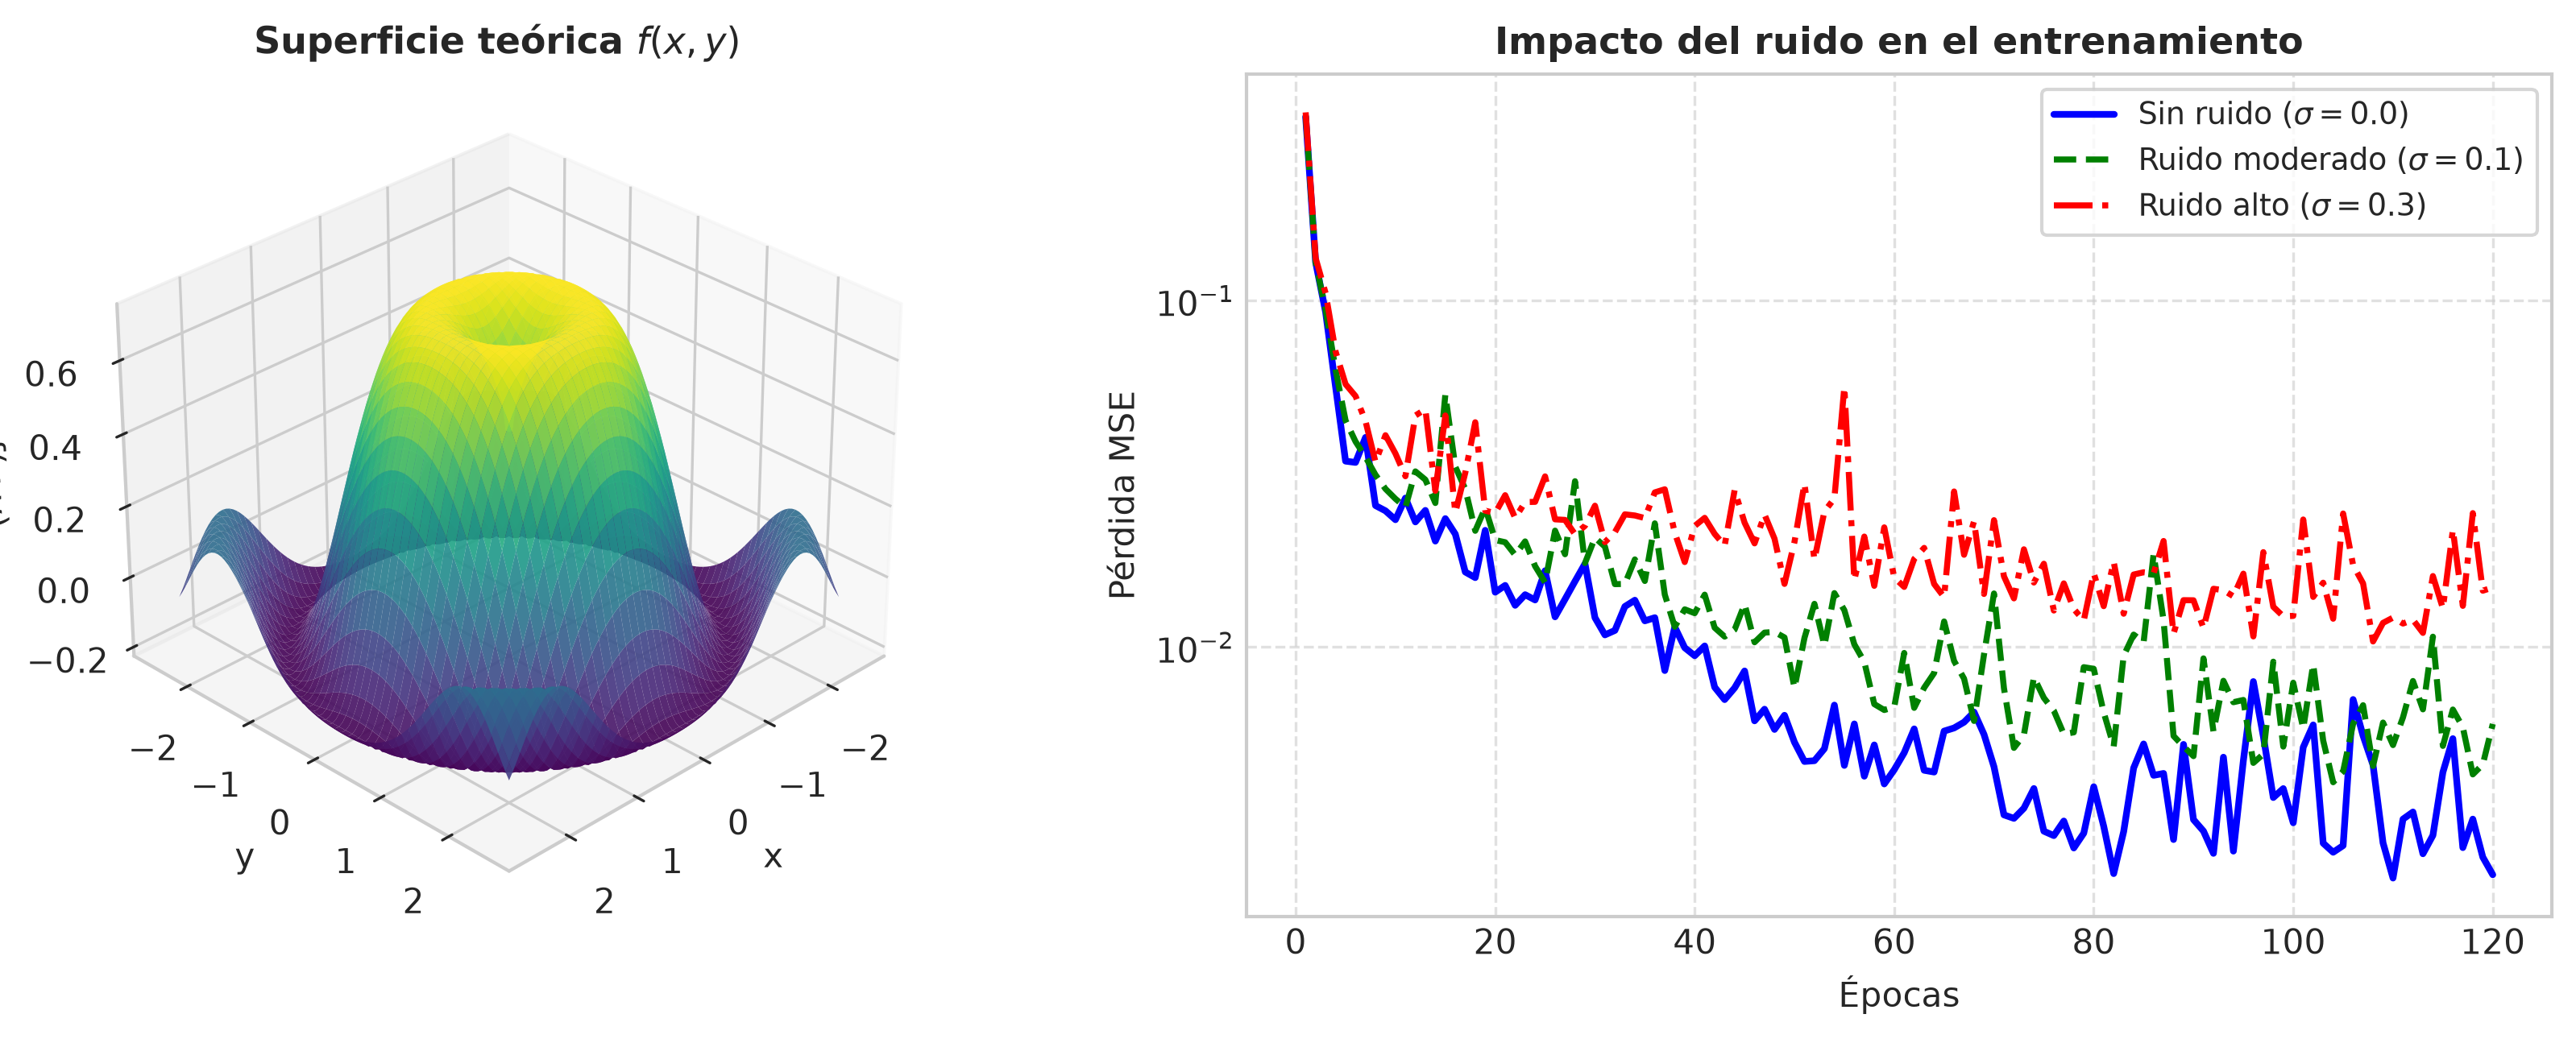
\includegraphics[height=3.0cm, keepaspectratio]{images/figura_2_superficie.png}
    \caption{Superficie objetivo y efecto del ruido. A la izquierda se ve el relieve tridimensional $f(x, y)$ con sus anillos ondulados. A la derecha se muestra cómo baja el error al entrenar la red con tres niveles de ruido ($\sigma = 0.0$, $\sigma = 0.1$ y $\sigma = 0.3$).}
    \label{fig:superficie}
\end{figure}

A la izquierda en la Figura~\ref{fig:superficie} vemos que esta función tiene un pico en el centro y varios anillos de valles y colinas a su alrededor, lo que genera zonas donde un optimizador simple se puede frenar.

\subsection*{¿Cuál es el impacto del parámetro de ruido en el proceso de optimización?}

El ruido proviene de las variaciones aleatorias en los datos y de calcular el gradiente usando muestras pequeñas (\textit{mini-batches}). En la gráfica de la derecha de la Figura~\ref{fig:superficie} se observa que tiene un doble efecto durante el entrenamiento: al comienzo resulta beneficioso porque las sacudidas ayudan a la red a no quedarse estancada en el primer valle o zona plana que encuentra, permitiéndole explorar y buscar mejores caminos. Sin embargo, al final del entrenamiento un nivel de ruido muy alto (curva roja) perjudica la precisión, ya que hace que los pesos bailen alrededor del mínimo sin poder asentarse en el valor óptimo. Por esta razón, en la práctica se suele reducir la tasa de aprendizaje progresivamente para explorar al inicio y lograr una convergencia fina al final.

\subsection*{¿Cómo se diferencia el método del descenso del gradiente con el descenso estocástico y las versiones aceleradas?}

Para comparar los optimizadores, entrenamos la red con cuatro métodos distintos, como se ve a la izquierda en la Figura~\ref{fig:optimizadores}:

\begin{figure}[H]
    \centering
    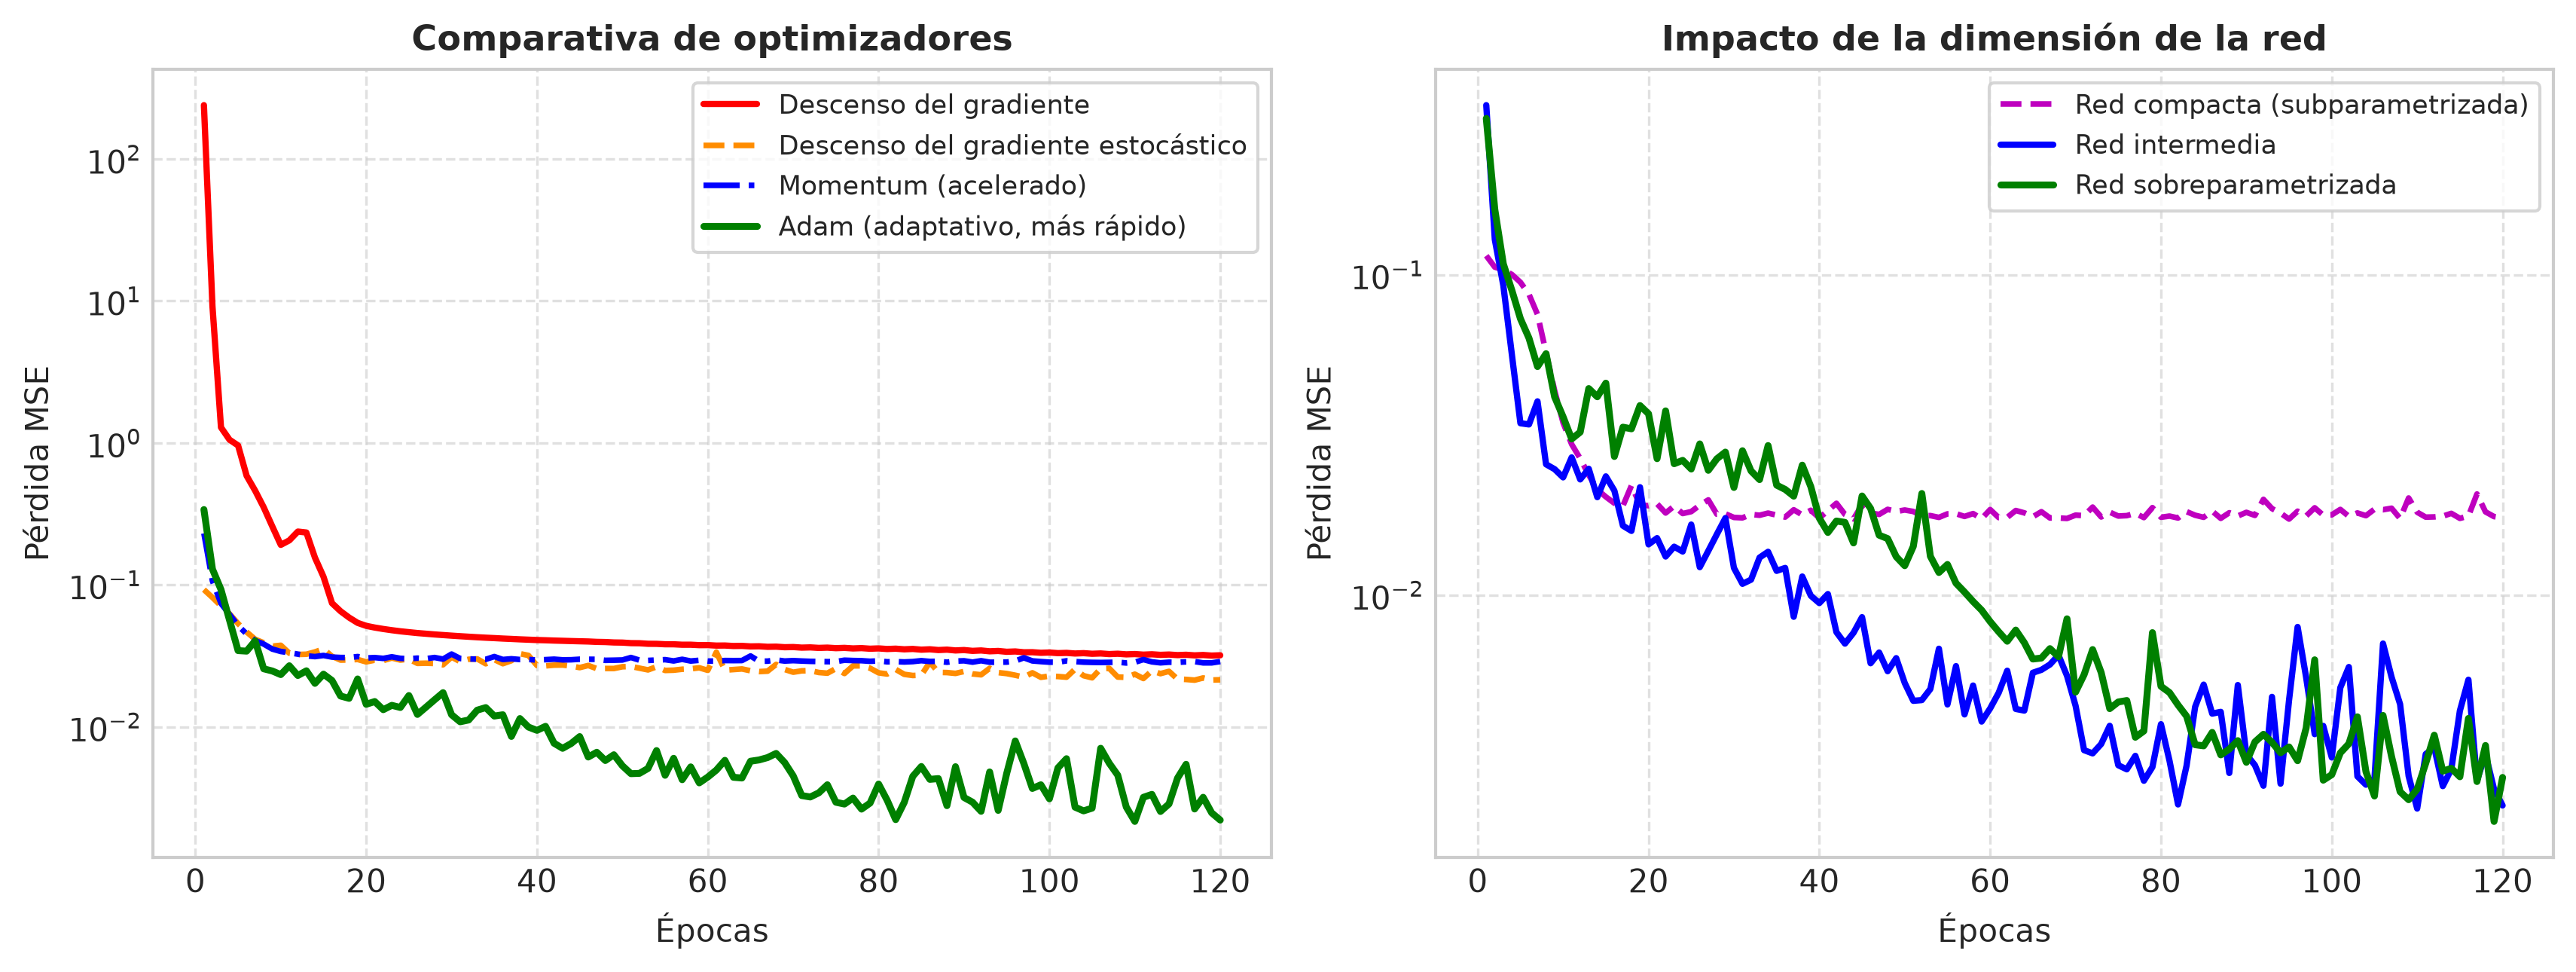
\includegraphics[height=3.0cm, keepaspectratio]{images/figura_3_optimizadores.png}
    \caption{Comparación de optimizadores y tamaño de la red. A la izquierda se muestra la rapidez con la que baja el error en cada método. A la derecha se compara el entrenamiento usando una red compacta, una intermedia y una grande.}
    \label{fig:optimizadores}
\end{figure}

Al analizar el comportamiento de cada método, encontramos diferencias fundamentales en su forma de cálculo, velocidad y estabilidad:
\begin{itemize}\itemsep-2pt \topsep0pt \partopsep0pt \parsep0pt
    \item \textbf{Descenso del gradiente:} Calcula el gradiente exacto usando todo el conjunto de entrenamiento para dar un solo paso. Aunque su trayectoria es muy suave y sin ruido, dar un único ajuste por época lo vuelve demasiado lento e ineficiente en tiempo real, además de que puede quedarse frenado con facilidad si cae en zonas planas o en mínimos locales.
    \item \textbf{Descenso del gradiente estocástico:} En vez de esperar a revisar todos los datos, divide el conjunto en grupos pequeños de 32 muestras y ajusta los pesos en cada grupo. Esto le permite hacer decenas de correcciones rápidas en una sola época, bajando el error mucho más rápido. Las pequeñas variaciones que introduce cada grupo generan sacudidas que le ayudan a no quedarse atascado en valles poco profundos.
    \item \textbf{Versiones con Momentum:} El descenso estocástico suele rebotar de lado a lado cuando el terreno tiene paredes muy empinadas y un fondo plano. Momentum corrige esto guardando una velocidad con los pasos anteriores. Como los rebotes van en direcciones opuestas se cancelan entre sí, mientras que el avance hacia adelante se va sumando, logrando que la red baje por el valle con mucha más rapidez y sin perder empuje en zonas planas.
    \item \textbf{Versiones aceleradas adaptativas como Adam:} Da un paso más allá al combinar el impulso de Momentum con un ajuste automático del paso para cada peso por separado. Si un peso viene cambiando con saltos muy bruscos, reduce su paso para no pasarse; si un peso casi no cambia en una zona plana, agranda su paso para avanzar más rápido. Gracias a esta doble adaptación, es el método más rápido, directo y estable para llegar al mínimo.
\end{itemize}

\subsection*{¿Cómo impacta la dimensión de la red neuronal en el rendimiento del optimizador?}

En la gráfica de la derecha de la Figura~\ref{fig:optimizadores} comparamos el entrenamiento usando redes de tres tamaños diferentes. Cuando la red es muy pequeña (curva morada), tiene pocos pesos y muy pocos grados de libertad; si cae en una zona con error alto, se queda atrapada fácilmente y se estanca por falta de capacidad. En cambio, cuando la red es más grande (curvas azul y verde), la gran cantidad de neuronas y parámetros crea muchísimas rutas libres para descender. En espacios de alta dimensión es casi imposible que el camino se cierre en todas las direcciones a la vez, por lo que el optimizador casi siempre encuentra una salida hacia abajo para seguir reduciendo el error hasta alcanzar una muy buena solución.

\subsection*{Diferencia entre épocas y tiempo de convergencia de los algoritmos}

Una época cuantifica el volumen de datos procesados (una pasada íntegra sobre el conjunto de entrenamiento), pero no refleja el esfuerzo computacional ni el tiempo transcurrido en el reloj. Por su parte, el tiempo de convergencia mide la duración temporal efectiva (segundos o minutos) que requiere el optimizador para alcanzar la cota de error deseada. En la práctica, mientras que el descenso del gradiente tradicional evalúa todo el conjunto para dar una sola actualización por época (resultando en un tiempo de reloj prohibitivo), métodos como SGD y Adam operan con mini-lotes (e.g. 32 muestras), realizando múltiples ajustes rápidos por época que reducen el tiempo total de convergencia de forma drástica.

{\setlength{\abovedisplayskip}{1pt}\setlength{\belowdisplayskip}{1pt}\setlength{\jot}{0pt}
\section*{II-C. Otros algoritmos de optimización}

\subsubsection*{1. AdamW (Decoupled Weight Decay)}
Corrige la interacción inadecuada entre la regularización $L_2$ y los momentos adaptativos de Adam: al agregar $\lambda \boldsymbol{\phi}_t$ al gradiente $\mathbf{g}_t$, la penalización se divide por $\sqrt{\tilde{\mathbf{v}}_t} + \epsilon$, reduciendo la regularización efectiva en parámetros frecuentes. AdamW desacopla la penalización y la aplica directamente a los pesos:
\begin{align*}
\mathbf{m}_{t+1} &= \beta \mathbf{m}_t + (1 - \beta) \mathbf{g}_t, \quad \tilde{\mathbf{m}}_{t+1} = \frac{\mathbf{m}_{t+1}}{1 - \beta^{t+1}} \\[0.01cm]
\mathbf{v}_{t+1} &= \gamma \mathbf{v}_t + (1 - \gamma) (\mathbf{g}_t \odot \mathbf{g}_t), \quad \tilde{\mathbf{v}}_{t+1} = \frac{\mathbf{v}_{t+1}}{1 - \gamma^{t+1}} \\[0.01cm]
\boldsymbol{\phi}_{t+1} &= (1 - \alpha \lambda) \boldsymbol{\phi}_t - \alpha \frac{\tilde{\mathbf{m}}_{t+1}}{\sqrt{\tilde{\mathbf{v}}_{t+1}} + \epsilon}
\end{align*}
El factor $(1 - \alpha \lambda)$ encoge uniformemente a $\boldsymbol{\phi}_t$ sin importar la curvatura ni la escala de cada coordenada.

\subsubsection*{2. AdaDelta (Adaptación basada en unidades de actualización)}
Supera la disminución monotónica de la tasa de aprendizaje en AdaGrad y la inconsistencia dimensional en las actualizaciones de parámetros. Emplea promedios móviles exponenciales de gradientes y de desplazamientos pasados:
\begin{align*}
\mathbf{v}_{t+1} &= \beta \mathbf{v}_t + (1 - \beta) (\mathbf{g}_t \odot \mathbf{g}_t), \quad \operatorname{RMS}[\mathbf{g}]_{t+1} = \sqrt{\mathbf{v}_{t+1} + \epsilon} \\[0.01cm]
\Delta \boldsymbol{\phi}_{t+1} &= - \frac{\operatorname{RMS}[\Delta \boldsymbol{\phi}]_t}{\operatorname{RMS}[\mathbf{g}]_{t+1}} \odot \mathbf{g}_t, \quad \boldsymbol{\phi}_{t+1} = \boldsymbol{\phi}_t + \Delta \boldsymbol{\phi}_{t+1} \\[0.01cm]
\mathbf{u}_{t+1} &= \beta \mathbf{u}_t + (1 - \beta) (\Delta \boldsymbol{\phi}_{t+1} \odot \Delta \boldsymbol{\phi}_{t+1}), \quad \operatorname{RMS}[\Delta \boldsymbol{\phi}]_{t+1} = \sqrt{\mathbf{u}_{t+1} + \epsilon}
\end{align*}
El paso se define por el cociente de magnitudes RMS, garantizando congruencia de unidades físicas.

\subsubsection*{3. RMSDrop / RMSProp (Root Mean Square Propagation)}
Evita la detención prematura de AdaGrad normalizando cada componente del gradiente mediante su promedio móvil cuadrático exponencial reciente ($\beta \approx 0.9$):
\begin{align*}
\mathbf{v}_{t+1} = \beta \mathbf{v}_t + (1 - \beta) (\mathbf{g}_t \odot \mathbf{g}_t), \quad \boldsymbol{\phi}_{t+1} = \boldsymbol{\phi}_t - \frac{\alpha}{\sqrt{\mathbf{v}_{t+1}} + \epsilon} \odot \mathbf{g}_t
\end{align*}

\subsubsection*{4. L-BFGS (Limited-memory Quasi-Newton)}
Aproxima el método de Newton ($\boldsymbol{\phi}_{t+1} = \boldsymbol{\phi}_t - \alpha_t \mathbf{H}_t^{-1} \mathbf{g}_t$) en tiempo y memoria lineal $\mathcal{O}(mD)$ sin calcular ni almacenar la Hessiana $\mathbf{H}_t$, guardando los desplazamientos de los últimos $m$ pasos ($\mathbf{s}_k = \boldsymbol{\phi}_{k+1} - \boldsymbol{\phi}_k$, $\mathbf{y}_k = \mathbf{g}_{k+1} - \mathbf{g}_k$, $\rho_k = 1 / (\mathbf{y}_k^T \mathbf{s}_k)$). El producto $\mathbf{r} = \mathbf{H}_t^{-1} \mathbf{g}_t$ se calcula mediante recursión en dos bucles:
\begin{itemize}\itemsep-3.5pt \parsep0pt \topsep0pt \partopsep0pt
    \item \textit{Bucle hacia atrás:} Para $k = t-1, \dots, t-m$: $\alpha_k = \rho_k \mathbf{s}_k^T \mathbf{q}$, $\mathbf{q} \leftarrow \mathbf{q} - \alpha_k \mathbf{y}_k$ (con $\mathbf{q} = \mathbf{g}_t$).
    \item \textit{Escalado y bucle hacia adelante:} $\mathbf{r} \leftarrow \frac{\mathbf{s}_{t-1}^T \mathbf{y}_{t-1}}{\mathbf{y}_{t-1}^T \mathbf{y}_{t-1}} \mathbf{q}$. Para $k = t-m, \dots, t-1$: $\beta_k = \rho_k \mathbf{y}_k^T \mathbf{r}$, $\mathbf{r} \leftarrow \mathbf{r} + \mathbf{s}_k (\alpha_k - \beta_k)$.
    \item \textit{Actualización de parámetros:} Dirección de descenso $\mathbf{d}_t = -\mathbf{r}$ y paso $\boldsymbol{\phi}_{t+1} = \boldsymbol{\phi}_t + \alpha_t \mathbf{d}_t$ con búsqueda de línea.
\end{itemize}
}

\clearpage
{\setlength{\abovedisplayskip}{1.5pt}\setlength{\belowdisplayskip}{1.5pt}\setlength{\intextsep}{1pt}\setlength{\abovecaptionskip}{1pt}\setlength{\belowcaptionskip}{1pt}
\section*{II-D. Inicialización}

\subsection*{Derivación analítica paso a paso de la inicialización de He y supuesto de activación}

Para analizar cómo cambia la varianza de la señal a medida que avanza por la red, consideramos dos capas consecutivas. Las preactivaciones de la capa previa son $\mathbf{f}$ (con dimensión $D_h$), las cuales pasan por la función de activación para dar $\mathbf{h} = a(\mathbf{f})$. La capa siguiente calcula sus nuevas preactivaciones $\mathbf{f}'$ sumando los sesgos y multiplicando los pesos por las activaciones entrantes:
\[
f'_i = \beta_i + \sum_{j=1}^{D_h} \Omega_{ij} h_j
\]
Siguiendo las indicaciones del problema y de la sección 7.5 del libro, fijamos todos los sesgos en cero ($\beta_i = 0$). Los pesos se eligen de forma aleatoria e independiente con una distribución normal de media cero y varianza $\sigma_\Omega^2$, es decir $\Omega_{ij} \sim \mathcal{N}(0, \sigma_\Omega^2)$, y asumimos además que no dependen de las activaciones entrantes $h_j$.

\textbf{1. Media de las nuevas preactivaciones:} Calculamos primero el valor promedio de la señal en la siguiente capa. Aplicando la propiedad de linealidad de la esperanza y recordando que los pesos tienen media cero y son independientes de las entradas:
\[
\mathbb{E}[f'_i] = \mathbb{E}\left[\sum_{j=1}^{D_h} \Omega_{ij} h_j\right] = \sum_{j=1}^{D_h} \mathbb{E}[\Omega_{ij}] \mathbb{E}[h_j] = \sum_{j=1}^{D_h} 0 \cdot \mathbb{E}[h_j] = 0
\]

\textbf{2. Varianza y anulación de términos cruzados:} Como la media es cero, la varianza es simplemente el promedio del cuadrado: $\operatorname{Var}[f'_i] = \mathbb{E}[(f'_i)^2]$. Desarrollando algebraicamente el cuadrado de la suma:
\begin{align*}
\operatorname{Var}[f'_i] &= \mathbb{E}\left[ \left( \sum_{j=1}^{D_h} \Omega_{ij} h_j \right)^2 \right] = \sum_{j=1}^{D_h} \mathbb{E}[\Omega_{ij}^2] \mathbb{E}[h_j^2] + \sum_{j=1}^{D_h} \sum_{k \neq j}^{D_h} \mathbb{E}[\Omega_{ij} \Omega_{ik}] \mathbb{E}[h_j h_k]
\end{align*}
Como los pesos de conexiones diferentes son independientes entre sí ($j \neq k$), su esperanza conjunta se factoriza como $\mathbb{E}[\Omega_{ij} \Omega_{ik}] = \mathbb{E}[\Omega_{ij}] \mathbb{E}[\Omega_{ik}] = 0 \cdot 0 = 0$. Por esta razón, todos los términos cruzados se anulan por completo. Sustituyendo la varianza de cada peso $\mathbb{E}[\Omega_{ij}^2] = \sigma_\Omega^2$, obtenemos directamente:
\[
\operatorname{Var}[f'_i] = \sum_{j=1}^{D_h} \sigma_\Omega^2 \mathbb{E}[h_j^2] = D_h \sigma_\Omega^2 \mathbb{E}[h_j^2]
\]

\textbf{3. Supuesto sobre la función de activación (ReLU):} ¿Qué supuesto sobre la activación se utiliza en esta derivación? Se asume que las preactivaciones de la capa anterior $f_j$ siguen una distribución simétrica alrededor de cero, con media cero ($\mathbb{E}[f_j] = 0$) y varianza $\sigma_f^2$. Esto significa que la probabilidad de que una entrada sea positiva o negativa es exactamente del 50\%. Al aplicar la función ReLU ($h_j = \max(0, f_j)$), todos los valores negativos se apagan a cero y los positivos quedan intactos. Calculamos el segundo momento $\mathbb{E}[h_j^2]$ integrando sobre la distribución:
\[
\mathbb{E}[h_j^2] = \int_{-\infty}^{\infty} (\max(0, z))^2 p(z) \, dz = \int_{0}^{\infty} z^2 p(z) \, dz = \frac{1}{2} \int_{-\infty}^{\infty} z^2 p(z) \, dz = \frac{1}{2} \operatorname{Var}[f_j] = \frac{1}{2} \sigma_f^2
\]

\textbf{4. Condición de preservación de varianza (Ecuación 7.31 de UDL):} Al sustituir $\mathbb{E}[h_j^2] = \frac{1}{2} \sigma_f^2$ en la varianza de $f'_i$, llegamos a la ecuación 7.31 del texto:
\[
\sigma_{f'}^2 = D_h \sigma_\Omega^2 \left( \frac{1}{2} \sigma_f^2 \right) = \frac{1}{2} D_h \sigma_\Omega^2 \sigma_f^2
\]
Para que la señal no se desvanezca hasta cero ni crezca de forma descontrolada al avanzar por capas profundas, exigimos que la varianza se conserve igual entre capas sucesivas ($\sigma_{f'}^2 = \sigma_f^2$). Igualando términos, despejamos directamente la regla de inicialización de He:
\[
\frac{1}{2} D_h \sigma_\Omega^2 = 1 \implies \sigma_\Omega^2 = \frac{2}{D_h} \implies \mathbf{\sigma_\Omega = \sqrt{\frac{2}{D_h}}}
\]

\textbf{5. Derivada y preservación del gradiente en el paso hacia atrás:} En el paso hacia atrás, aplicamos la regla de la cadena para derivar la función de pérdida respecto a la preactivación previa:
\[
\frac{\partial \ell}{\partial f_{k-1, j}} = \sum_{i=1}^{D_{\text{out}}} \frac{\partial \ell}{\partial f_{k, i}} \frac{\partial f_{k, i}}{\partial h_j} \frac{\partial h_j}{\partial f_{k-1, j}} = \sum_{i=1}^{D_{\text{out}}} \Omega_{ij} \frac{\partial \ell}{\partial f_{k, i}} \mathbb{I}(f_{k-1, j} > 0)
\]
donde $\mathbb{I}(f_{k-1, j} > 0)$ es la derivada de la función ReLU (vale 1 si la preactivación es positiva y 0 si es negativa). Por la simetría de la entrada, la derivada vale 1 la mitad de las veces, por lo que la varianza del gradiente retropropagado también conserva el factor de un medio: $\operatorname{Var}\left[\frac{\partial \ell}{\partial f_{k-1, j}}\right] = \frac{1}{2} D_{\text{out}} \sigma_\Omega^2 \operatorname{Var}\left[\frac{\partial \ell}{\partial f_k}\right]$, lo que daría $\sigma_\Omega^2 = \frac{2}{D_{\text{out}}}$ si calibráramos en la dirección de retroceso.

\subsection*{Inicialización Xavier / Glorot para activación sigmoide y comparación con He}

\textbf{¿Por qué el supuesto de He deja de ser válido para la sigmoide de la Figura 1?}
La función sigmoide $\sigma(z) = \frac{1}{1 + e^{-z}}$ siempre devuelve valores positivos en el intervalo $(0, 1)$, por lo que su valor medio no es cero sino $\mathbb{E}[h] \approx 0.5 \neq 0$. Además, la sigmoide nunca corta las activaciones a cero exacto, por lo que no existe el apagado del 50\% y el factor $\frac{1}{2}$ desaparece por completo. Cerca del origen ($z \approx 0$), la sigmoide opera en su zona lineal con pendiente suave, de modo que las activaciones conservan directamente la dispersión de las entradas: $\operatorname{Var}[h_j] \approx \operatorname{Var}[f_j]$.

\textbf{Derivación analítica de Xavier hacia adelante y hacia atrás:}
En el paso hacia adelante (\textit{forward}), al no existir el recorte a la mitad, la varianza transmitida por una capa con $D_{\text{in}}$ entradas es $\operatorname{Var}[f'_i] = \sum_{j=1}^{D_{\text{in}}} \sigma_\Omega^2 \operatorname{Var}[h_j] \approx D_{\text{in}} \sigma_\Omega^2 \operatorname{Var}[f_j]$. Exigir que la señal conserve su escala unitaria hacia adelante impone $D_{\text{in}} \sigma_\Omega^2 = 1 \implies \sigma_{\Omega, \text{fwd}}^2 = \frac{1}{D_{\text{in}}}$.

En el paso hacia atrás (\textit{backward}), usamos la regla de la cadena para derivar la pérdida respecto a la preactivación previa con la derivada de la sigmoide $\sigma'(t) = \sigma(t)(1 - \sigma(t))$, y calculamos la varianza del gradiente retropropagado:
\begin{align*}
\frac{\partial \ell}{\partial f_{k-1, j}} &= \sum_{i=1}^{D_{\text{out}}} \frac{\partial \ell}{\partial f_{k, i}} \frac{\partial f_{k, i}}{\partial f_{k-1, j}} = \left( \sum_{i=1}^{D_{\text{out}}} \Omega_{ij} \frac{\partial \ell}{\partial f_{k, i}} \right) \sigma'(f_{k-1, j}) \\[0.05cm]
\operatorname{Var}\left[\frac{\partial \ell}{\partial f_{k-1, j}}\right] &= \sum_{i=1}^{D_{\text{out}}} \mathbb{E}[\Omega_{ij}^2] \operatorname{Var}\left[\frac{\partial \ell}{\partial f_{k, i}}\right] = D_{\text{out}} \sigma_\Omega^2 \operatorname{Var}\left[\frac{\partial \ell}{\partial f_k}\right]
\end{align*}
Para evitar que los gradientes se desvanezcan o exploten al retroceder capa por capa, se exige $D_{\text{out}} \sigma_\Omega^2 = 1 \implies \sigma_{\Omega, \text{bwd}}^2 = \frac{1}{D_{\text{out}}}$.

\textbf{¿Por qué Xavier promedia entrada y salida mientras que He solo usa la de entrada?}
Cuando una capa tiene diferente número de entradas y salidas ($D_{\text{in}} \neq D_{\text{out}}$), ninguna varianza puede cumplir ambas condiciones simultáneamente. Glorot y Bengio resuelven este dilema calculando la media armónica entre ambas condiciones:
\[
\sigma_\Omega^2 = \frac{2}{\frac{1}{\sigma_{\Omega, \text{fwd}}^2} + \frac{1}{\sigma_{\Omega, \text{bwd}}^2}} = \frac{2}{D_{\text{in}} + D_{\text{out}}} \implies \mathbf{\sigma_\Omega = \sqrt{\frac{2}{D_{\text{in}} + D_{\text{out}}}}}
\]
En cambio, en redes con activación ReLU, el corte del 50\% ocurre exactamente igual hacia adelante ($h = \max(0, f)$) que hacia atrás ($\frac{\partial h}{\partial f} = \mathbb{I}(f > 0)$). Ambas direcciones comparten el mismo factor 2 en el numerador ($\sigma_{\text{fwd}}^2 = 2/D_{\text{in}}$ y $\sigma_{\text{bwd}}^2 = 2/D_{\text{out}}$). Por esta razón, calibrar los pesos únicamente con las neuronas de entrada ($\sigma_\Omega = \sqrt{2/D_{\text{in}}}$) asegura un paso hacia adelante balanceado, y en el paso hacia atrás los gradientes sólo cambian por la proporción de dimensiones $\prod \frac{D_{\text{in}}}{D_{\text{out}}}$, la cual permanece acotada y estable sin necesidad de promediar la salida.

\subsection*{Cálculo numérico de $\sigma_\Omega$ para cada capa de la red de la Figura 1}
Evaluamos analíticamente ambas fórmulas para cada matriz de pesos de la red ($2 \to 3 \to 2 \to 1$):
\vspace{-0.1cm}
\begin{table}[H]
\centering
\footnotesize
\renewcommand{\arraystretch}{0.72}
\setlength{\tabcolsep}{4pt}
\begin{tabular}{lccccc}
\toprule
\textbf{Capa} & $D_{\text{in}}$ & $D_{\text{out}}$ & \textbf{Fórmula de He} & \textbf{Fórmula de Xavier} & \textbf{Valores numéricos} \\
\midrule
Capa 0 ($\boldsymbol{\Omega}_0$) & 2 & 3 & $\sqrt{2/2} = 1.0$ & $\sqrt{2/(2+3)} = \sqrt{0.4}$ & $\sigma_{\text{He}} = \mathbf{1.0000}, \; \sigma_{\text{Xavier}} \approx \mathbf{0.6325}$ \\
Capa 1 ($\boldsymbol{\Omega}_1$) & 3 & 2 & $\sqrt{2/3} \approx 0.8165$ & $\sqrt{2/(3+2)} = \sqrt{0.4}$ & $\sigma_{\text{He}} \approx \mathbf{0.8165}, \; \sigma_{\text{Xavier}} \approx \mathbf{0.6325}$ \\
Capa 2 / Salida ($\boldsymbol{\Omega}_2$) & 2 & 1 & $\sqrt{2/2} = 1.0$ & $\sqrt{2/(2+1)} = \sqrt{2/3}$ & $\sigma_{\text{He}} = \mathbf{1.0000}, \; \sigma_{\text{Xavier}} \approx \mathbf{0.8165}$ \\
\bottomrule
\end{tabular}
\end{table}
\vspace{-0.15cm}

\subsection*{Comportamiento en redes profundas ($K \ge 20$ capas) y práctica del Notebook 7.3}
A partir del Notebook 7.3 construimos una red profunda de 20 capas ocultas ($D=80$, ReLU) para evaluar experimentalmente la evolución de la varianza hacia adelante y la magnitud de los gradientes hacia atrás (Figura~\ref{fig:inicializacion}):
\begin{figure}[H]
    \centering
    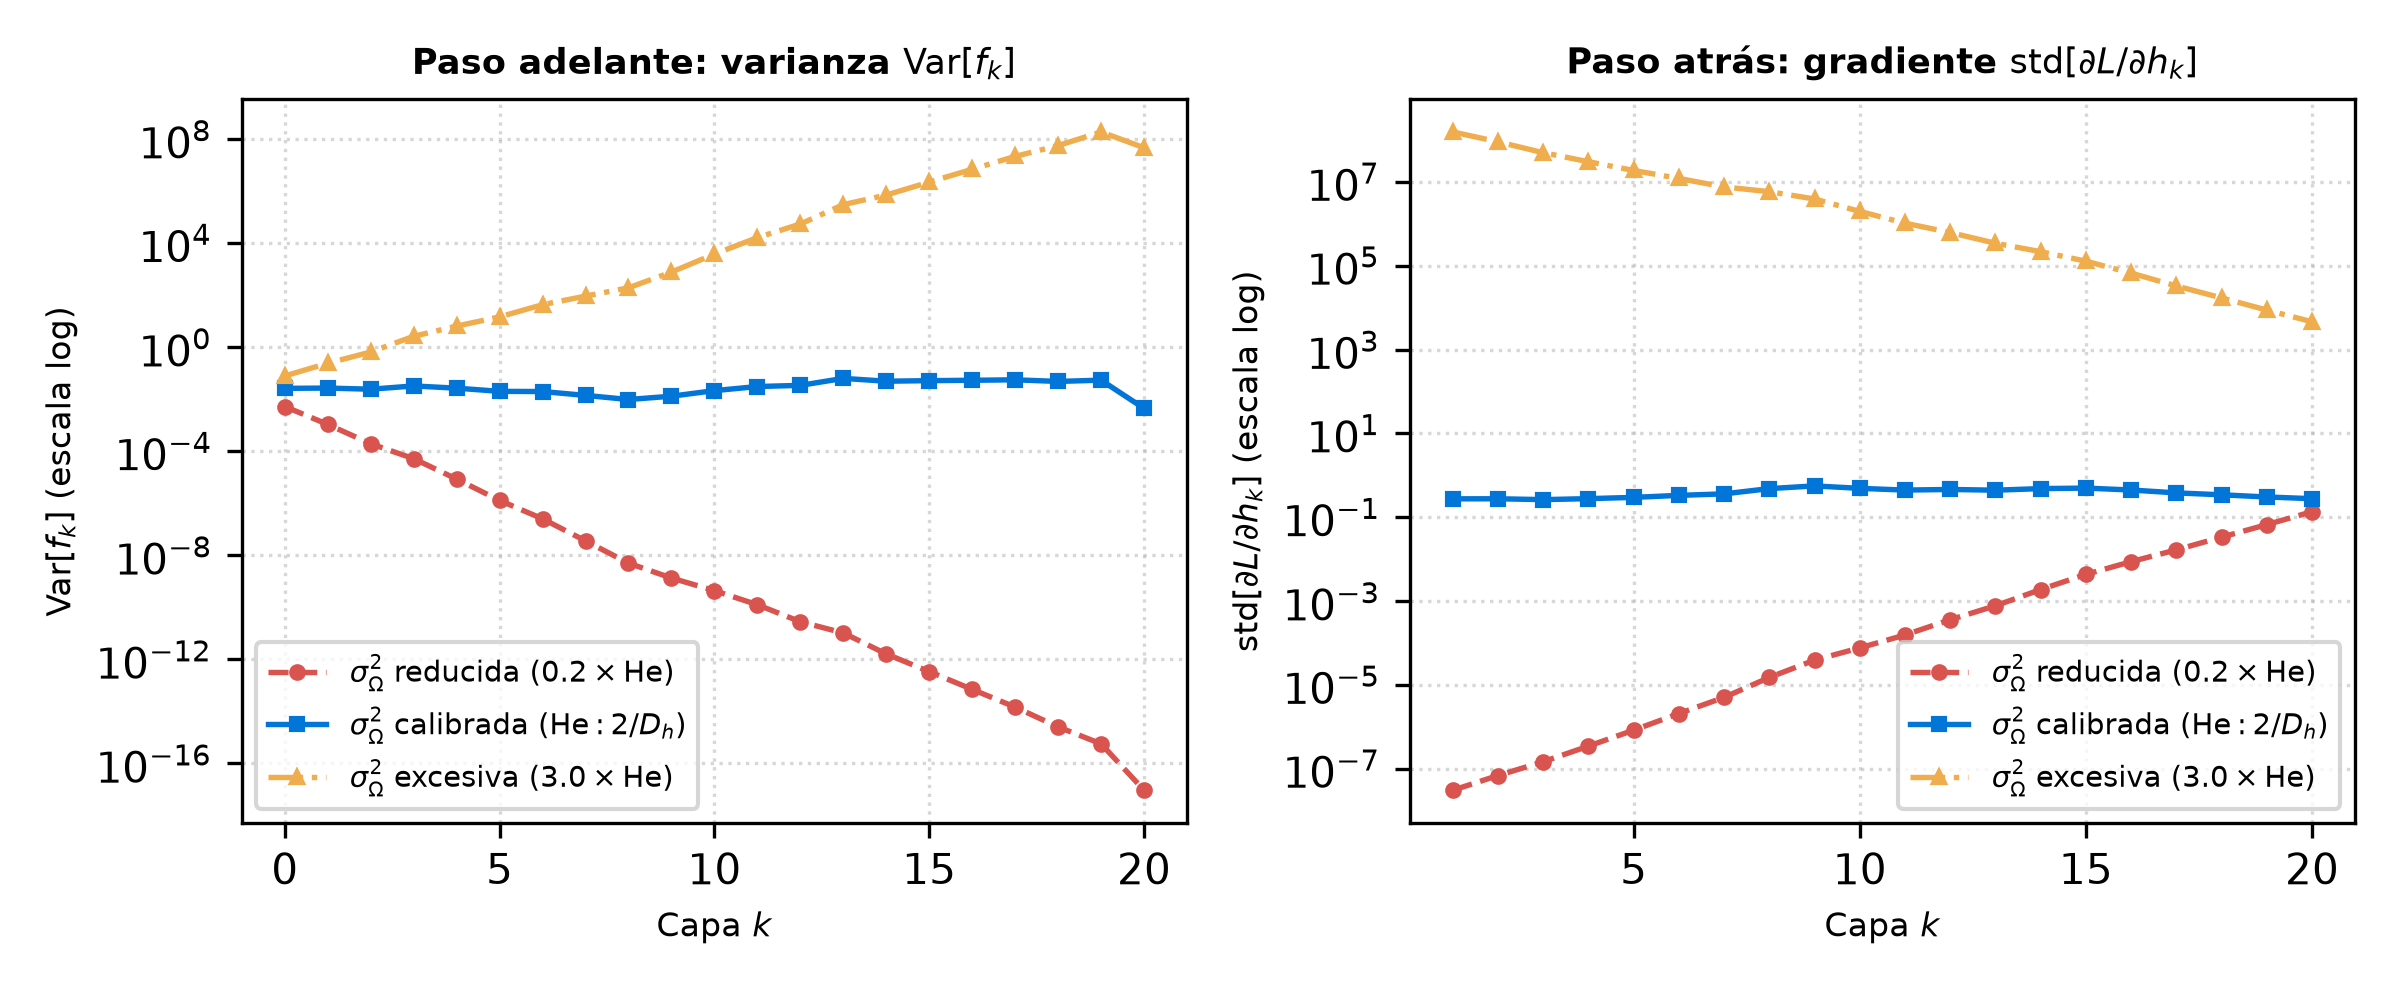
\includegraphics[height=3.0cm, keepaspectratio]{images/figura_4_inicializacion.png}
    \caption{Simulación en red profunda de 20 capas ($D=80$, ReLU) del Notebook 7.3. Izquierda: evolución de la varianza en el paso hacia adelante. Derecha: desviación estándar de los gradientes retropropagados.}
    \label{fig:inicializacion}
\end{figure}

El análisis de las curvas experimentales muestra el impacto directo de la inicialización en el entrenamiento profundo. Cuando la varianza es insuficiente ($0.2 \times \text{He}$), la señal se apaga hasta colapsar ($\operatorname{Var}[f_{20}] \approx 10^{-17}$) y los gradientes retropropagados caen a $10^{-8}$ en las primeras capas, provocando un severo desvanecimiento del gradiente (\textit{vanishing gradients}) que frena el aprendizaje. Si la varianza es excesiva ($3.0 \times \text{He}$), la señal se amplifica superando $10^7$ y los gradientes se disparan a $10^8$, desatando una explosión del gradiente (\textit{exploding gradients}) y saturación numérica (\textit{NaN}). En cambio, la inicialización de He ($2/D_h$) conserva la varianza ($\approx 0.02$) y la escala de gradientes ($\approx 0.35$) estables a lo largo de las 20 capas, garantizando un aprendizaje profundo balanceado y confiable.
}

\end{document}